% !Mode::"TeX:UTF-8"
% !Mode:: "TeX:UTF-8"
\documentclass[xcolor=svgnames,serif,table,10pt]{beamer}
\mode<presentation>{
% Setup appearance:
\useoutertheme{infolines}
\usetheme{Darmstadt}
\setbeamercovered{transparent}
\setbeamertemplate{caption}[numbered]
\setbeamertemplate{navigation symbols}{}
\setbeamertemplate{blocks}[rounded][shadow=true]
\setbeamertemplate{enumerate items}[circle]

% 修改样式
\setbeamercolor{box}{bg=black!20!orange,fg=white}
\setbeamercolor{block title}{use=sidebar,fg=sidebar.fg!10!white,bg=orange!70!black}
\setbeamercolor{block title example}{use=sidebar,fg=sidebar.fg!10!white,bg=black!60!green}
\setbeamercolor{block title alerted}{use=sidebar,fg=sidebar.fg!10!white,bg=black!50!red}

\setbeamertemplate{headline}
{%
  \begin{beamercolorbox}[shadow=true]{section in head/foot}
  \vskip2pt\insertnavigation{\paperwidth}\vskip2pt
  \end{beamercolorbox}%
}
}
\usepackage{url}
\usepackage{animate}
\usepackage[english]{babel}
\usepackage{times}
\usepackage[T1]{fontenc}
\usepackage{multirow,multicol,longtable}
\usepackage{graphics}
\usepackage{xcolor}
\usepackage[no-math]{fontspec}%-------------------------------------------------- 提供字体选择命令
\usepackage{xunicode}%----------------------------------------------------------- 提供Unicode字符宏
\usepackage{xltxtra}%------------------------------------------------------------ 提供了针对XeTeX的改进并且加入了XeTeX的LOGO
\usepackage[BoldFont,SlantFont,CJKchecksingle]{xeCJK}%--------------------------- 使用xeCJK宏包


%================================== 设置中文字体 ================================%
%\setCJKmainfont{Adobe Heiti Std}%------------------------------------------------设置正文为黑体
%\setCJKmonofont{Adobe Song Std}%-------------------------------------------------设置等距字体
%\setCJKsansfont{Adobe Kaiti Std}%------------------------------------------------设置无衬线字体
% \setCJKfamilyfont{zxzt}{FZShouJinShu-S10S}
% \setCJKfamilyfont{FZDH}{FZDaHei-B02S}
%================================== 设置中文字体 ================================%

%================================== 设置英文字体 ================================%
\setmainfont[Mapping=tex-text]{Times New Roman}%--------------------------------英文衬线字体
\setsansfont[Mapping=tex-text]{Arial}%------------------------------------英文无衬线字体
\setmonofont[Mapping=tex-text]{Courier New}%-------------------------------------英文等宽字体
\newfontfamily\Arial{Arial}
%================================== 设置英文字体 ================================%

%================================== 设置数学字体 ================================%
%\setmathsfont(Digits,Latin,Greek)[Numbers={Lining,Proportional}]{Minion Pro}
%================================== 设置数学字体 ================================%
\punctstyle{kaiming}%------------------------------------------------------------ 开明式标点格式
\usepackage{graphicx}
\usepackage{tikz}
\usetikzlibrary{positioning,backgrounds}
\usetikzlibrary{fadings}
\usetikzlibrary{patterns}
\usetikzlibrary{calc}
\usetikzlibrary{shadings}
\pgfdeclarelayer{background}
\pgfdeclarelayer{foreground}
\pgfsetlayers{background,main,foreground}
\usepackage{xifthen}
\usepackage{colortbl,dcolumn}
\usepackage{enumerate}
\usepackage{pifont}
\usepackage{tabularx}
\usepackage{booktabs}
\usepackage{hyperref}
%=================================== 数学符号 =================================%
\newcommand{\rtn}{\mathrm{\mathbf{R}}}
\newcommand{\N}{\mathrm{\mathbf{N}}}
\newcommand{\As}{\mathrm{a.s.}}
\newcommand{\Ae}{\mathrm{a.e.}}
\newcommand*{\PR}{\mathrm{\mathbf{P}}}
\newcommand*{\EX}{\mathrm{\mathbf{E}}}
\newcommand{\EXlr}[1]{\mathrm{\mathbf{E}}\left[#1\right]}
\newcommand*{\dif}{\,\mathrm{d}}
\newcommand*{\F}{\mathcal{F}}
\newcommand*{\h}{\mathcal{H}}
\newcommand*{\vp}{\varepsilon}
\newcommand*{\prs}{\dif\PR-\As}
\newcommand*{\dte}{\dif t-\Ae}
\newcommand*{\pts}{\dif\PR\times\dif t-\Ae}
\newcommand{\Ito}{It\^{o}}
\newcommand{\tT}[1][0]{[#1,T]}
\newcommand{\intT}[2][T]{\int^{#1}_{#2}}
\newcommand{\intTe}[1][t]{\intT[t+\varepsilon]{#1}}
\newcommand{\s}{\mathcal{S}}
\newcommand{\me}{\mathrm{e}}
\newcommand{\one}[1]{{\bf 1}_{#1}}
\renewcommand{\M}{{\rm M}}
\newcommand{\Me}[1][t]{M^{\varepsilon}_{#1}}
\newcommand{\Ne}[1][t]{N^{\varepsilon}_{#1}}
\newcommand{\Pe}[1][t]{P^{\varepsilon}_{#1}}
\DeclareMathOperator*{\sgn}{sgn}
% =================================== 数学符号 =================================%

% 定义罗马数字
\makeatletter
\newcommand{\rmnum}[1]{\romannumeral #1}
\newcommand{\Rmnum}[1]{\expandafter\@slowromancap\romannumeral #1@}
\makeatother

% 定义破折号
\newcommand{\pozhehao}{\kern0.3ex\rule[0.8ex]{2em}{0.1ex}\kern0.3ex}
% 中文日期
\def\CJK@today{\the\year 年 \the\month 月}
\newcommand\zhtoday{\CJK@today}

% 中文图表
\renewcommand\figurename{图}
\renewcommand\tablename{表}

\graphicspath{{./}}

% Author, Title, etc.

\title{信号检测与估值}

%% \subtitle{Foreground-constrained Eulerian Video Motion Magnification}

\author[段江涛]{段江涛
\\机电工程学院}

\institute[LSEC,AMSS,CAS]{
\includegraphics[height=1cm]{xd.jpg}}

\date{\zhtoday}

\setlength{\baselineskip}{22pt}
\renewcommand{\baselinestretch}{1.4}

% The main document

\begin{document}
\setlength{\abovedisplayskip}{1ex}%------------------------------------------ 公式前的距离
\setlength{\belowdisplayskip}{1ex}%------------------------------------------ 公式后的距离

\begin{frame}
  \titlepage
\end{frame}

\begin{frame}
  \frametitle{主要内容}
  \tableofcontents[hideallsubsections]
\end{frame}

\section{随机变量}

\begin{frame}
随机事件的特征是不确定性,但是我们可以通过重复观测,从不确定现象中寻找、观察特定事件发生的规律,为此需要让某一随机现象重复发生(不一定是人为控制的)并记录观测结果,称之为随机试验。

随机试验的三个特征:
\begin{itemize}
	\item 可以在相同条件下重复进行;
	\item 试验的所有可能结果是明确可知的,并且不止一个;
	\item 每次试验总是恰好出现这些可能结果中的一个,但在一次试验之前却不能肯定这次试验会出现哪个结果。
\end{itemize}

\end{frame}

\begin{frame}

概率论中的三个组成部分:
\begin{itemize}
	\item 样本空间$\Omega$
	\item 事件域$\mathcal{F}$
	\item 概率$P$
\end{itemize}
\end{frame}


\begin{frame}
\begin{itemize}
	\item 样本空间$\Omega$:一个随机试验所有可能出现的结果的全体,称为随机事件的样本空间。\\
	每一个可能的结果称为基本事件,它们的全体就是样本空间。
	\item 样本点$\xi_k$:随机试验的一个结果,就是某个基本事件,也就是$\Omega$中的一个元素。\\
	$\Omega=\{\xi\}=\{\xi_k|k=1,\dots,n\}$
	\item 随机事件$A$: 样本空间中的某个子集称为随机事件,简称事件(事件是集合)。
    \item 事件域$\mathcal{F}$: 样本空间中的某些子集构成的满足如下条件的集合,称为事件域(又称$\sigma^-$域)。
	\begin{itemize}
		\item[(1)] $\Omega\in\mathcal{F}$
		\item[(2)] 若$A\in\mathcal{F}$, 则$A$的补$\overline{A}\in\mathcal{F}$
		\item[(3)] 若$A_n\in\mathcal{F}$, 则$\bigcap_{n=1}^{\infty}\in\mathcal{F}$
	\end{itemize}
\end{itemize}
\end{frame}

\begin{frame}
\begin{example}
	一个盒子中有10个相同的球,5各白色,5个黑色,搅匀后从中任意摸取一球。\\
	$\xi_1=\{\text{取得白球} \}$, $\xi_2=\{\text{取得黑球} \}$\\
	$\Omega=\{\xi_1,\xi_2\}$
\end{example}
\begin{example}
	一个盒子中有10个相同的球,编号1,2,...,10, 从中取一球。\\
	$\Omega=\{1,2,\dots,10\}$\\
	$A=\{\text{6号球} \}=\{6\}$, $B=\{\text{偶数编号球} \}=\{2,4,6,8,10\}$, $\overline{B}=\{\text{奇数编号球}\}$,$C=\{\text{编号小于等于5的球} \}=\{1,2,3,4,5\}$\\
	事件A是基本事件,而B和C则由多个基本事件所组成,并且$A,B,C\subset\Omega$。
\end{example}
\textit{空集$\emptyset$可以看作$\Omega$的子集,在任意一次试验中不可能有此事件发生,称为不可能事件。}
\end{frame}

\begin{frame}
  事件域中的元素就是随机事件。如果这些事件的随机性能够由定义在$\mathcal{F}$上的具有非负性,归一性和可列加性的实函数$P(A)$来确定,则称$P$是定义在二元组$(\Omega,\mathcal{F})$上的概率,而称$P(A)$为事件$A$的概率。
  \begin{enumerate}
  	\item[(1)] 非负性。 $P(A)\ge 0$
  	\item[(2)] 归一性。 $P(\Omega)=1$
    \item[(3)] 可列加性。$A_1,A_2,...,A_n$互不相容$(A_i\cap A_j=\emptyset,i\ne j)$,则$P(A_1\cup A_2\cup\dots\cup A_n) = P(A_1)+P(A_2)+\cdots+P(A_n)$
  \end{enumerate}
\end{frame}

\begin{frame}
	非空的事件域$\mathcal{F}$关于交、并、补、差元素是封闭的。
	\begin{enumerate}
		\item 若$A\in\mathcal{F}$, 则$\overline{A}\in\mathcal{F}$
		\item 若$A\in\mathcal{F},B\in\mathcal{F}$, 则$A\cup B\in \mathcal{F}$
		\item 若$A\in\mathcal{F},B\in\mathcal{F}$, 则$A\cap B\in \mathcal{F}$
		\item 若$A\in\mathcal{F},B\in\mathcal{F}$, 则$A- B\in \mathcal{F}$
	\end{enumerate}
	\begin{proof}
		由于$\mathcal{F}$为非空子集类,则若$A\in\mathcal{F}$,由(1)知,$\overline{A}\in\mathcal{F}$,又由(2)知$A\cup\overline{A}=\Omega\in\mathcal{F}$. 故有$\Omega\in\mathcal{F}$. \\
		若$A\in\mathcal{F},B\in\mathcal{F}$, 则$\overline{A}\in\mathcal{F}$, $\overline{B}\in\mathcal{F}$,那么$\overline{A}\cup\overline{B}\in\mathcal{F}$, 即有$A\cap B=\overline{\overline{A}\cup\overline{B}}\in\mathcal{F}$,故$\mathcal{F}$对交也封闭。\\
		再若$A,B\in\mathcal{F}$, 则有$A-B=A\overline{B}\in\mathcal{F}$, 即$\mathcal{F}$对交也封闭。\\
		由数学归纳法可证,若$A_i\in\mathcal{F}$, 则$\bigcup_{i=1}^{n}\in\mathcal{F}$
	\end{proof}
\end{frame}

\begin{frame}
\frametitle{古典概型}
\begin{itemize}
	\item 样本空间的元素(即基本事件)只有有限个,不妨设为$n$个,$\Omega=\{\xi_1,\xi_2,\dots,\xi_n\}$
	\item 每个基本事件出现的可能性是相等的,即有$P(\xi_1)=P(\xi_2)=\cdots=P(\xi_n)$
	\item 事件域$\mathcal{F}$为$\Omega$的所有子集的全体,即是$Pwr(\Omega),\Omega$的m幂集,共有$2^n$个事件,$\emptyset\in\mathcal{F},\Omega\in\mathcal{F}$。
	\item 由概率的有限可加性知\\
	$1=P(\Omega)=\Sigma_{i=1}^{n}P(\xi_i)\implies P(\xi_i)=\frac{1}{n},(i=1,\dots,n)$
	\item 对任意一个随机事件$A\subseteq\mathcal{F}$, 如果$A$是$k$个基本事件的和,即$A=\{\xi_{i_1}\}\cup \{\xi_{i_2}\}\cup\cdots\cup\{\xi_{i_k}\}$, 则
	$$P(A)=\frac{k}{n}=\frac{\text{$A$中所包含的基本事件数}}{\text{基本事件总数}}$$
\end{itemize}
\end{frame}

\begin{frame}
\frametitle{样本空间的选取}
为求一个事件的概率,样本空间可以有不同的取法,但一定要认真,基本事件和求概事件数的计算都要在同一个样本空间中进行,否则会导致谬误!
\begin{example}
	一个盒子中有10个相同的球,编号1,2,...,10, 从中取一球,求此球的号码为偶数的概率。\\
	$\Omega=\{1,2,\dots,10\}$\\
	$A=\{\text{偶数编号球} \}=\{2\}\cup\{4\}\cup\{6\}\cup\{8\}\cup\{10\}=\{2,4,6,8,10\}$。\\
	$P(A)=\frac{|A|}{n}=\frac{5}{10}=\frac{1}{2}$
\end{example}
另外一种解法:$\Omega=\{A,\overline{A}\},A=\{\text{编号为偶数的球}\},\overline{A}=\{\text{编号为奇数的球}\},\mathcal{F}=\{\emptyset,\Omega,A,\overline{A}\}$,由$A,\overline(A)$的对称性,即得$P(A)=\frac{1}{2}$

\end{frame}

\begin{frame}
\frametitle{样本空间的选取}
\begin{block}{Notes}
	两种解法的样本空间$\Omega$不同(从而事件域$\mathcal{F}$是不同的)。严格地说,两者所描述的随机试验是不同的。例如对于第二种解法来说,$B=\{\text{号码为4的球}\}$并不属于事件域$\mathcal{F}$,就是说$B$不是一个事件,从而也就没有概率可言。但对第一种解法,$B$是事件,而且$P(B)=\frac{1}{10}$。
\end{block}

\end{frame}

\begin{frame}
\begin{example}
	甲、乙两人掷硬币,其中甲掷$n+1$次,乙掷$n$次。求``甲掷出正面的次数大于乙指出正面的次数"这一事件的概率。\\
	令\\ $A_1=$甲掷出正面的次数,$A_2=$甲掷出反面的次数,$B_1=$乙掷出正面的次数,$B_2=$乙掷出反面的次数。\\
	$\Omega-\{A_1 > B_1\}=\{A_2\le B_1\}=\{A_2>B_2\}$\\
	由对称性知\\
	$P(A_1>B_1)=P(A_2>B_2)$\\
	由此即得\\
	$P(A_1>B_1)=\frac{1}{2}$
\end{example}
\begin{block}{Notes}
	在古典概型中,所谓``等可能性'',正是``对称性"产生的结果,因为各个基本事件处在``对称"的位置上,所以才有``等可能性"。
\end{block}
\end{frame}

\begin{frame}{几何概率}
我们在一个面积为$S_\Omega$的区域$\Omega$中,等可能地任意投点,如果点落入小区域$S_A$中的可能性与$S_A$成正比,而与$A$的位置及形状无关。如果``点落入小区域$A$"这个随机事件仍然记为$A$,则由$P(\Omega)=1$可得
$$P(A)=\frac{S_A}{S_\Omega}$$
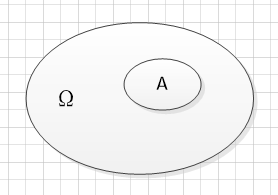
\includegraphics[scale=0.4]{geometry}
\end{frame}

\begin{frame}
\begin{example}
	(会面问题)甲、乙两人约定在6时到7时之间在某处会面,并约定先到者应等候另一个人一刻钟,过时即可离去。求两人能会面的概率。\\
	如图,以x,y表示甲乙两人,则两人能会面的充要条件是: $|x-y|\leq 15$\\
	$$P(A)=\frac{S_A}{S_\Omega}=\frac{60^2-45^2}{60^2}=\frac{7}{16}$$
	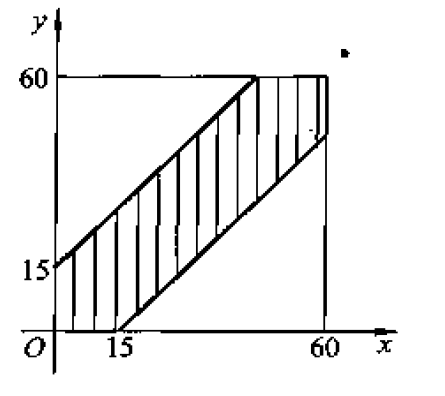
\includegraphics[scale=0.4]{geometry1}
\end{example}
\end{frame}

\section{条件概率}

\begin{frame}{条件概率}
\begin{definition}
	若$\Omega,\mathcal{F},P$是一个概率空间,$B\in\mathcal{F}$, 且$P(B)>0$,则对任意的$A\in\mathcal{F}$,称
	$$P(A|B)=\frac{P(AB)}{P(B)}$$
	为在已知事件B发生的条件下,事件A发生的条件概率。
\end{definition}
\begin{corollary}
概率的乘法公式:  $P(AB=P(B)P(A|B)$
\end{corollary}

\begin{corollary}
	$P(A_1A_2\cdots A_n)=P(A_1)P(A_2|A_1)P(A_3|A_1A_2)\cdots P(A_n|A_1A_2\cdots A_{n-1})$
\end{corollary}
\end{frame}

\begin{frame}
\begin{example}
	一个家庭中有两个小孩,乙指其中有一个是女孩,问这是另一个小孩也是女孩的概率有多大?\\
	$\Omega=$\{(男,男),(男,女),(女,男),(女,女)\}\\
	$A=$\{已知有一个是女孩\}=\{(男,女),(女,男),(女,女)\}\\
	$B=$\{另一个也是女孩\}=\{(女,女)\}\\
	于是所求概率为\\
	$P(B|A)=\frac{P(AB)}{P(A)}=\frac{1/4}{3/4}=\frac{1}{3}$
\end{example}
\end{frame}

\begin{frame}
\begin{example}
	有外形相同的球分装在三个盒子,每盒10个。其中第一个盒子中7个球标有字母A,3个球标有字母B; 第二个盒子中有红球和白球各5个; 第三个盒子中则有红球8个,白球2个。试验按如下规则进行: 先在第一个盒子中任取一个球,若取得标有字母A的球,则在第二个盒子中任取一个球; 若第一次取得标有字母B的球,则在第三个盒子中任取一个球。如果第二次取出的是红球,则称试验成功。求试验成功的概率。
\end{example}
\end{frame}

\begin{frame}
\begin{solution}
	令$A=$\{从第一个盒子取得标有字母A的球\},$B=$\{从第一个盒子取得标有字母B的球\},$R=$\{第二次取出的球是红球\},$W=$\{第二次取出的球是白球\}。\\
	则容易球得: $P(A)=\frac{7}{10}, P(B)=\frac{3}{10}, P(R|A)=\frac{1}{2},P(W|A)=\frac{1}{2},P(R|B)=\frac{4}{5},P(W|B)=\frac{1}{5}$\\
	于是,试验成功的概率为
	\begin{align*}
	P(R)=P(R\cap\Omega)&=P[R\cap(A\cup B)]\\
	&=P(RA\cup RB)=P(RA)+P(RB)\\
	&=P(R|A)\cdot P(A)+P(R|B)\cdot P(B)\\
	&=\frac{1}{2}\cdot\frac{7}{10}+\frac{4}{5}\cdot\frac{3}{10}=0.59
	\end{align*}
	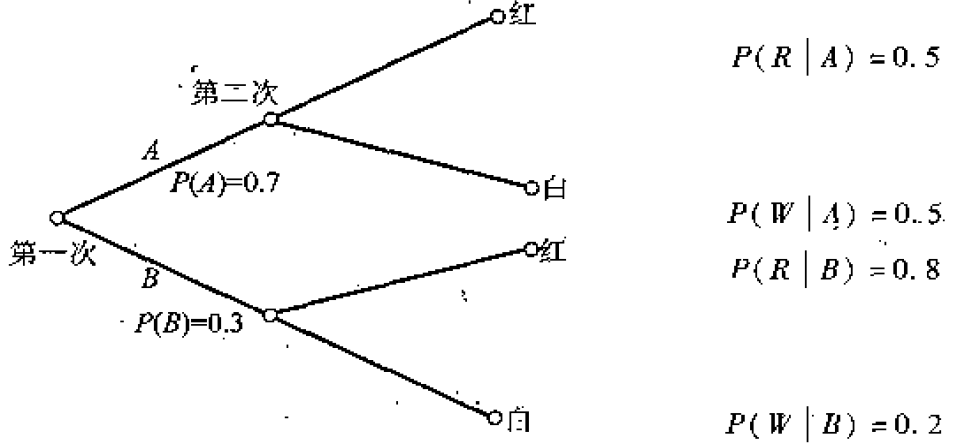
\includegraphics[scale=0.18]{tree}
\end{solution}
\end{frame}

\begin{frame}{概率树/全概率公式}
概率树思想:为了求解复杂事件的概率,往往可以先把它分解成两个(或若干个)互不相容的较简单的事件之并。求出这些较简单事件的概率,在利用加法公式即得所要求的复杂事件的概率。把这个方法一般化,便的到下述定理。
\begin{theorem}
	设$B_1,B_2,\cdots$是一列互不相容的事件,且有
	\[\bigcup_{i=1}^{+\infty}B_i=\Omega,P(B_i)>0 \]
	则对任一事件A,有
	\[P(A)=\sum_{i=1}^{+\infty}P(B_i)P(A|B_i) \]	
\end{theorem}
\end{frame}

\begin{frame}{概率树/全概率公式}
\begin{proof}
	\begin{align*}
	P(A)&=P(A\cap\Omega)=P[A\cap(\bigcup_{i=1}^{+\infty}B_i)]\\
	&=P[\bigcup_{i=1}^{+\infty}(AB_i)]=\sum_{i=1}^{+\infty}P(AB_i)\\
	&=\sum_{i=1}^{+\infty}P(B_i)P(A|B_i)
	\end{align*}
\end{proof}
\end{frame}

\begin{frame}{相互独立事件}
\begin{definition}
对任意的两个事件A,B,若
\[P(AB)=P(A)P(B)\]
成立,则称事件A,B是相互独立的,简称为独立的。	
\end{definition}
\begin{block}{依这个定义,不难验证:}
	若A与B相互独立,则$\{\emptyset,A,\overline{A},\Omega\}$中的任意一个与$\{\emptyset,B,\overline{B},\Omega\}$中的任意一个仍相互独立。
\end{block}
\end{frame}

\section{随机变量}

\begin{frame}
\begin{definition}
	设$(\Omega,\mathcal{F},P)$是一概率空间,$x(\xi)|\xi\in\Omega$是定义在$\Omega$上的单值实函数,如果对任一实数$x$, 集合$\{x(\xi)\le x\}\in\mathcal{F}$, 则称$x(\xi)$为$(\Omega,\mathcal{F},P)$上的一个\textbf{随机变量}。
	
	随机变量$x(\xi)$的定义域为样本空间$\Omega$,它的值域是实数R。所有随机变量$x(\xi)$实际上是一个映射,这个映射为每个来自概率空间的结果(样本点)$\xi$赋予一个实数$x$。这种映射必须满足条件:
	\begin{itemize}
		\item[(1)] 对任一$x$,集合$\{x(\xi)\le x\}$是这个概率空间中的一个事件,并有确定的概率$P\{x(\xi)\le x\}$;
		\item[(2)] $P\{x(\xi)=\infty \}=0$, $P\{x(\xi)=-\infty \}=0$
	\end{itemize}
	\begin{block}{Notes}
		随机变量就是试验结果(即样本点)和实数之间的一一对应关系。
	\end{block}
\end{definition}
\end{frame}

\begin{frame}
关于随机变量(及向量)的研究,是概率论的中心内容.这是因为,对于一个随机试验,我们所关心的往往是与所研究的特定问题有关的某个或某些量,而这些量就是随机变量.

也可以说:\textbf{随机事件}是从静态的观点来研究随机现象,而\textbf{随机变量}则是一种动态的观点,一如数学分析中的常量与变量的区分那样.变量概念是高等数学有别于初等数学的基础概念。同样,概率论能从计算一些孤立事件的概念发展为一个更高的理论体系,其基础概念是随机变量。
\end{frame}

\begin{frame}
\begin{example}
	抛硬币试验中,H表示正面,T表示反面,样本空间$\Omega=\{H,T\}$,H与T不是数量,不便于计算及理论的研究,因而引入以下变量$\xi$,
	$$x=x(\xi)=
	\begin{cases}
	0, &\xi=T\\
	1, &\xi=H
	\end{cases}
	$$
\end{example}  
\end{frame}

\begin{frame}
\begin{definition}
设随机试验E的样本空间是$\Omega=\{\xi\}$, 若对于每一个$\xi\in\Omega$,有一个实数$x(\xi)$与之对应,即$x(\xi)$是定义在$\Omega$上的单值函数,称为随机变量。
\end{definition}
\begin{figure}[htbp]
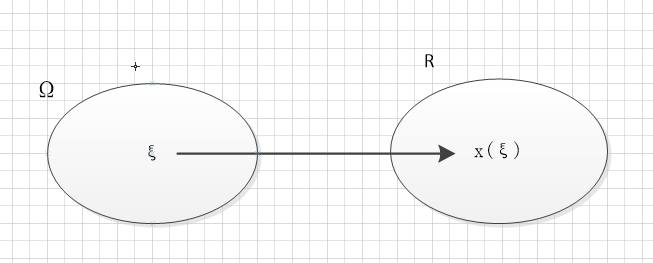
\includegraphics[scale=0.3]{xi_map}
\end{figure}
\begin{itemize}
\item 可用随机变量$x(\xi)$描述事件。\\
例掷一颗骰子(色子),设出现的点数记为随机事件A,表示``掷出的点数大于3''的事件A,可表示为``$x(\xi)>3$''。反过来,A的一个变化范围表示一个随机事件:``$2<x(\xi)<5$''表示事件``掷出的点数大于2且小于5''。
\item 随机变量随着试验的结果而取不同的值,在试验之前不能确切知道它取什么值,但是随机变量的取值有一定的统计规律性---概率分布。
\end{itemize}
\end{frame}


\begin{frame}{研究随机变量的意义}
  虽然在试验之前不能肯定随机变量$x(\xi)$会取哪一个数值,但是对于任一实数$a$,我们可以研究$\{x(\xi)=a\}$发生的概率,也就是$x(\xi)$取值的统计规律。
\end{frame}
\begin{frame}{离散型随机变量}
	\begin{definition}
		定义在样本空间$\Omega$上,取值于实数域$R$,且只取有限个或可列个值的变量$x=x(\xi)$, 称作是一维离散型随机变量。
	\end{definition}
	\begin{example}
		设$\Omega=$\{某公司2018年对某险种售出的保单\}, 对$\xi\in\Omega$, 令
		\[x(\xi)=\xi\text{在一年中的索赔次数}\]
		则$x(\xi)$是$\Omega$上的一个一位离散型随机变量, $x(\xi)$的可能取值范围为$\{0,1,2,\dots\}$。 在试验(即签定某一份保单)之前,并不能断定$\xi$会取哪一个值,但是我们可以知道$(\xi=0),(\xi=1),\dots$这些事件发生的概率(也就是在总体中所占的比例)。制表称为随机变量$x(\xi)$的分布。
		\begin{tabular}{|c|c|c|c|}
			\hline 
			$\xi$ & 0 & 1 & $\cdots$\\ 
			\hline 
			$P(\xi)$ & $p_1$ & $p_2$ & $\cdots$\\ 
			\hline 
		\end{tabular} 
	\end{example}
\end{frame}
\begin{frame}
\begin{example}
	某射手命中率为$p,(0<p<1)$,现有五发子弹。射击一发,如果命中,即停止射击,否则再射击一次,依次类推,如用$\eta$表示他射击所用去的子弹数,求$\eta$的分布。\\
	当$(\eta=k),1\le k\le 4$时表示前$(k-1)$次射击均未命中。第$k$次才首次命中,依题意,每次射击是相互独立的。故$P(\eta=k| 1\le k\le 4)=(1-p)^{k-1}p$。而$(\eta=5)$时表示前4次射击均为命中,第5次射击后不管是否命中均要停止。故$P(\eta=k|k=5)=(1-p)^{k-1}p$。\\
	\begin{tabular}{|c|c|c|c|c|c|}
		\hline 
		$\eta$ & 1 & 2 & 3 & 4 & 5\\ 
		\hline 
		$P(\eta)$ & $p$ & $p(1-p)$ & $p(1-p)^2$ & $p(1-p)^3$  & $(1-p)^4$ \\ 
		\hline 
	\end{tabular} 
\end{example}
\end{frame}
\begin{frame}{离散型随机变量$\xi$的分布列的性质}
\begin{block}{离散型随机变量$\xi$的分布列}
	\begin{tabular}{|c|c|c|c|}
		\hline 
		$\xi$ & 0 & 1 & $\cdots$\\ 
		\hline 
		$P(\xi)$ & $p_1$ & $p_2$ & $\cdots$\\ 
		\hline 
	\end{tabular} 
\end{block}

由概率的性质可知,任一离散型随机变量的分布$\{p_i\}$都有下述两个性质:
\begin{enumerate}
	\item $p_i\ge 0,i=1,2,...$
	\item $\sum_{i=1}^{+\infty}{p_i}=1$.
\end{enumerate}
反过来,任意一个具有以上两个性质的数列$\{p_i\}$,都有资格作为某一个随机变量的分布列。
\end{frame}

\begin{frame}
分布列不仅明确地给出了$(\xi=a_i)$的概率,而且对于任意一个的实数a,b,事件$(a\le\xi\le b)$发生的概率均可由分布列算出,因为
\[(a\le\xi\le b)=\bigcup_{a\le\xi\le b}(\xi=a_i)\]
于是由概率的可列加性有
\[P(a\le\xi\le b)=\sum_{i\in I_{a,b}}P(\xi=a_i)=\sum_{i\in I_{a,b}}p_i\]
其中$I_{a,b}=\{i:a\le a_i\le b\}$,即使对$\mathbb{R}$中更复杂可列的集合$B$,也有
\[P(\xi\in B)=\sum_{i\in I(B)}P(\xi=a_i)=\sum_{i\in I(B)}p_i\]
其中$I(B)=\{i:a_i\in B\}$\\
由知此可,$x(\xi)$取各种值的概率都可以由它的分布列通过计算而得到。
\begin{block}{}
	分布列全面地描述了离散型随机变量$x(\xi)$的统计规律。
\end{block}
\end{frame}

\section{几种重要的离散型随机变量的分布}
\begin{frame}
\begin{definition}[0--1分布]
	若$x(\xi)$的概率分布是\\
	\begin{center}
	\begin{tabular}{|c|c|c|}
		\hline 
		$\xi$ & 0 & 1\\ 
		\hline 
		$P(\xi)$ & $1-p$ & $p$\\ 
		\hline 
	\end{tabular} \\
	\end{center}
	则称$x(\xi)$服从参数$p$的0--1分布。
\end{definition}
\begin{example}
	一批产品的废品率为5\%, 从中任取一个进行检查, 若令$\xi$表示取得废品的数量,写出$\xi$的概率分布。\\
	\begin{tabular}{|c|c|c|}
		\hline 
		$\xi$ & 0 & 1\\ 
		\hline 
		$P(\xi)$ & $0.95$ & $0.05$\\ 
		\hline 
	\end{tabular} 
\end{example}
\end{frame}
\begin{frame}
\begin{definition}[几何分布]
	若$x(\xi)$的概率分布是
	\[P(\xi=k)=(1-p)^{k-1}p,\qquad (0<p<1,k=1,2,\dots)\]
	则称$x(\xi)$服从参数为$p$的几何分布,记作$\xi\sim G(p)$
\end{definition}
\end{frame}

\begin{frame}
\begin{example}
	社会上定期发行某种奖券,每券一元,中奖率为$p$,某人每次购买1张奖券, 如果没有中奖,下次继续购买一张,直到中奖为止。求该人购买奖券次数$\xi$的概率分布。\\
	令$A_k=$\{第$k$次购买的奖券中奖\}, $k=1,2,3,...$, \\
	则$P(A_k)=p,\quad P(\overline{A_k})=1-p$, \\
	由于$A_1,A_2,A_3,\dots$相互独立,于是:
	\begin{align*}
	P(\xi=1)&=P(A_1)=p\\
	P(\xi=2)&=P(\overline{A_1}A_1)=P(\overline{A_1})P(A_2)=(1-p)p\\
	P(\xi=3)&=P(\overline{A_1}\overline{A_2}A_3)=P(\overline{A_1})P(\overline{A_2})P(A_3)=(1-p)^{2}p\\
	\cdots\\
	P(\xi=k)&=P(\overline{A_1}\overline{A_2}\cdots\overline{A_{k-1}}A_k)=P(\overline{A_1})P(\overline{A_2})\cdots P(\overline{A_{k-1}})P(A_k)=(1-p)^{k-1}p
	\end{align*}
\end{example}
\end{frame}

\begin{frame}
\begin{block}{二项分布}
	若试验E只有两种可能结果,一种是事件A出现,另一种是事件$\overline{A}$出现,$P(A)=p$, 称试验E为伯努利(Bernoulli)试验。现将试验E独立重复n次,若用$\xi$表示事件A出现的次数,在这n重伯努利试验中,事件A恰好出现k次的概率为
	\[P\{\xi=k\}=C_{n}^{k}p^{k}(1-p)^{n-k},\qquad k=0,1,2,\dots,n\]
\end{block}
\begin{definition}[二项分布]
	若$\xi$的概率分布是
	\[P\{\xi=k\}=C_{n}^{k}p^{k}(1-p)^{n-k},\qquad k=0,1,2,\dots,n\]
	则称$\xi$服从参数为n,p的二项分布,记作$\xi\sim B(n,p)$。
\end{definition}
\end{frame}

\begin{frame}
\begin{example}
	一批产品的废品率为0.03,进行20次独立重复抽样,求出现废品的频率为0.1的概率。\\
	令$\xi$表示在这20次独立重复抽样中出现的废品数,则$\xi\sim B(20,0.03)$。于是
	\[P\{\frac{\xi}{20}=0.1\}=P\{\xi=2\}=C_{20}^{2}0.03^{2}(0.97)^{18}\approx 0.0988\]
\end{example}
\end{frame}
\section{第三部分}
\begin{frame}
  一些内容
\end{frame}
\begin{frame}
  一些内容
\end{frame}




\begin{frame}[plain]{}
  \begin{center}
    \begin{tikzpicture}
      \node[above,xscale=1.2,yscale=1.2]{\Huge 欢迎批评指正!};
    \end{tikzpicture}
  \end{center}
\end{frame}

\end{document}






%%%%下面的内容不参与文档的编译。使用者在想用某个东西时直接可通过查阅,并复制黏贴和修改使用。

\iffalse  %注释开始

%垂直居中
\begin{frame}
  \begin{center}
  需要居中的内容!
  \end{center}
\end{frame}
或者
\begin{frame}
  \centering
  一些内容
\end{frame}

%幻灯片标题的使用
\begin{frame}
\frametitle{第一部分第一张幻灯}
  一些内容
\end{frame}

%项目编号的使用
\begin{frame}
  \frametitle{条目}
  \begin{itemize}
  \item 项目1
  \item 项目2
  \item 项目3
  \item 项目4
    \begin{itemize}
    \item 二级项目1
    \item 二级项目2
    \end{itemize}
  \end{itemize}
\end{frame}

%表格的使用
\begin{frame}
  \frametitle{表格}
  \begin{table}[htbp!]
    \centering
    \caption{主流机器学习框架}
    \begin{tabular}{c|c|c|c|c}
      \toprule[1pt]
      机器学习库	& 机构 & 支持语言  & 平台 & Tensor \\
      \toprule[1pt]
      TensorFlow	& Google & C++,Python &跨平台 & Good \\
 	  \hline
      Pytorch	&  Facebook& Python & 跨平台 & Good \\
 	  \bottomrule[1pt]
    \end{tabular}
  \end{table}
\end{frame}

%区块的使用
\begin{frame}
  \frametitle{分析}
  \begin{block}{XXX 算法}
	\begin{itemize}
		\item 步骤1
	 	\item 步骤2
	 	\item 步骤3
	 \end{itemize}
  \end{block}
\end{frame}

%使用区块来强调内容
\begin{frame}
  \frametitle{强调}
  \begin{itemize}
  \item 这是内容
  \end{itemize}
  \only<1>\begin{block}{}
    这里蹦出来一个强调!
  \end{block}
\end{frame}

%section中目录的使用
\begin{frame}
  \frametitle{技术影响力}
    \tableofcontents[currentsection,hideallsubsections]
\end{frame}

%插入图片
\begin{frame}
\begin{figure}[!h]
  \centering
  % Requires \usepackage{graphicx}
  \includegraphics[width=2cm]{pics/logo.jpg}\\
  \caption{logo图片样例}\label{pic6}
\end{figure}
\end{frame}

%分栏实现图文混排
\begin{frame}
分栏前面的一些内容!!
\begin{columns}%0.6 0.4表示相对比例
\column{0.6\textwidth}%<1->
分栏的左侧,文字叙述。
\column{0.4\textwidth}%<1->
分栏的右侧插入了图片。
 \begin{figure}[!h]
  \centering
  % Requires \usepackage{graphicx}
  \includegraphics[width=4cm]{pics/logo.jpg}\\
  \caption{logo图片样例}\label{pic6}
\end{figure}
\end{columns}
分栏后面的一些内容!!
\end{frame}

\fi   %注释结束
